%%%%%%%%%%%%%%%%%%%%%%%%%%%%%%%%%%%%%%%%%
% a0poster Portrait Poster
% LaTeX Template
% Version 1.0 (22/06/13)
%
% The a0poster class was created by:
% Gerlinde Kettl and Matthias Weiser (tex@kettl.de)
% 
% This template has been downloaded from:
% http://www.LaTeXTemplates.com
%
% License:
% CC BY-NC-SA 3.0 (http://creativecommons.org/licenses/by-nc-sa/3.0/)
%
%%%%%%%%%%%%%%%%%%%%%%%%%%%%%%%%%%%%%%%%%

%----------------------------------------------------------------------------------------
%	PACKAGES AND OTHER DOCUMENT CONFIGURATIONS
%----------------------------------------------------------------------------------------

\documentclass[a0,portrait]{a0poster}
\usepackage[ngerman]{babel}
\usepackage[backend=biber,style=numeric]{biblatex}
\addbibresource{sample.bib}
\usepackage{multicol} % This is so we can have multiple columns of text side-by-side
\columnsep=100pt % This is the amount of white space between the columns in the poster
\columnseprule=3pt % This is the thickness of the black line between the columns in the poster

\usepackage[svgnames]{xcolor} % Specify colors by their 'svgnames', for a full list of all colors available see here: http://www.latextemplates.com/svgnames-colors

\usepackage{times} % Use the times font
%\usepackage{palatino} % Uncomment to use the Palatino font

\usepackage{graphicx} % Required for including images
\graphicspath{{figures/}} % Location of the graphics files
\usepackage{booktabs} % Top and bottom rules for table
\usepackage[font=small,labelfont=bf]{caption} % Required for specifying captions to tables and figures
\usepackage{amsfonts, amsmath, amsthm, amssymb} % For math fonts, symbols and environments
\usepackage{wrapfig} % Allows wrapping text around tables and figures

\begin{document}

%----------------------------------------------------------------------------------------
%	POSTER HEADER 
%----------------------------------------------------------------------------------------

% The header is divided into two boxes:
% The first is 75% wide and houses the title, subtitle, names, university/organization and contact information
% The second is 25% wide and houses a logo for your university/organization or a photo of you
% The widths of these boxes can be easily edited to accommodate your content as you see fit

\begin{minipage}[b]{0.75\linewidth}
\veryHuge \color{Green} \textbf{Prototyping} \color{Black}\\ % Title
\Huge\textit{Ein Poster in der Vorlesung "Forschungsmethoden"}\\[2cm] % Subtitle
    \huge \textbf{Sajedeh Majdi \& Amin Beikzadeh \& Christian Rebischke}\\[0.5cm] % Author(s)
\huge Technische Universität Clausthal\\[0.4cm] % University/organization
\Large sajedeh.majdi@tu-clausthal.de, amin.beikzadeh@tu-clausthal.de, christian.rebischke@tu-clausthal.de\\
\end{minipage}
%
\begin{minipage}[b]{0.25\linewidth}

\includegraphics[width=20cm]{Logo_TUC_de_CMYK.pdf}\\
\end{minipage}

\vspace{1cm} % A bit of extra whitespace between the header and poster content

%----------------------------------------------------------------------------------------

\begin{multicols}{2} % This is how many columns your poster will be broken into, a portrait poster is generally split into 2 columns

%----------------------------------------------------------------------------------------
%	ABSTRACT
%----------------------------------------------------------------------------------------

\color{Green} % Navy color for the abstract

\begin{abstract}
Um den teilnehmenden Studenten verschiedene Methoden zur Erhebung und Auswertung von Daten näher zu bringen, bietet die Technische Universität Clausthal die Vorlesung "Forschungsmethoden" an. Dieses Poster soll einen Überblick über das "Prototyping", einen Teilbereich dieser Methoden, darstellen. Im Prototyping wird versucht möglichst frühzeitig erste Ergebnisse zu einer Forschungsfrage zu erhalten, in dem die Durchführbarkeit oder die Eignung des Forschungsobjekts direkt anhand eines praktischen Beispiels getestet wird, ein Prototyp.
In unserem Poster möchten wir mögliche Gründe für ein Prototyping erläutern, sowie dessen Vor- und Nachteile erläutern, und einige Beispiele zum Prototyping nennen.
\end{abstract}

%----------------------------------------------------------------------------------------
%	INTRODUCTION
%----------------------------------------------------------------------------------------

\color{Black} % SaddleBrown color for the introduction

\section*{Einleitung}
Ein Prototyp, vom griechischen Wort "protos" "der Erste" und "typos" "Urbild" oder "Vorbild", ist ein Modell zum Beweisen und/oder Veranschaulichen einer wissenschaftlichen Hypothese. Die genaue Gestalt diesen Prototypen ist abhängig von der wissenschaftlichen Fachrichtung. In der "Physik" beispielsweise kann ein Prototyp, der praktische Beweis einer physikalischen Gleichung sein. In der "Chemie" wiederum kann ein Prototyp eine neuartige künstlich erschaffene Substanz sein. Auf die "Informatik" bezogen ist mit Prototyp allerdings meist entweder eine Hardware, Software oder eine Verbindung aus beiden gemeint. Der Vorgang der Erstellung eines solchen Prototypen nennt sich "Prototyping". Nachfolgend wollen wir das Prototyping anhand von Gründen, Beispielen und bekannter Vor- und Nachteile näher erläutern.
%----------------------------------------------------------------------------------------
%	OBJECTIVES
%----------------------------------------------------------------------------------------

\color{Black} % DarkSlateGray color for the rest of the content

\section*{Gründe für ein Prototyping}
Ein Prototyp stellt meistens ein vereinfachtes, nicht fertiges System oder Modell dar[3], um die Machbarkeit einer wissenschaftlichen Hypothese zu testen. Demnach begründet sich ein Prototype im Drang eine theoretische Frage anhand eines praktischen Beispiels zu testen, zu erläutern oder zu verstehen. Außerdem kann ein Prototyp geschaffen werden um sich frühzeitig Feedback zum Forschungsthema zu verschaffen. Dieses Feedback kann entweder am Ende der Prototyping-Phase erhalten werden oder bereits während des Baus des Prototypen können Methoden eingesetzt werden um Feedback zu erhalten, welche dann den Bau des Prototypen beeinflussen. Prototypen kommen meistens dann zum Einsatz, wenn ein praktischer Beweis einer Theorie besonders günstig oder naheliegend erscheint. Weitere Gründe für einen Protoypen ist die höhere Akzeptanz und Verständlichkeit eines physischen oder virtuellen Modells. Beispiel dazu ist das Gesetz der Schwerkraft (Physik) und dem Versuchsaufbau, welcher die Schwerkraft misst oder besser veranschaulicht.


%----------------------------------------------------------------------------------------
%	MATERIALS AND METHODS
%----------------------------------------------------------------------------------------

\section*{Vorteile}
Mögliche Vorteile von Prototyping sind:
\begin{itemize}
    \item Eine kontinuierliche Weiterentwicklung eines praktischen Beispiels zum Stützen einer These bis zum vollendeten Produkt (dies ist besonders Interessant bei Forschungsaufträgen aus der Industrie).
    \item Das abschließende Finden und Beheben von Fehlern in der theoretischen Ausarbeitung einer Forschung, welche in der Theorie als klein eingestuft worden sind, aber in der Praxis eine große Rolle spielen. Zum Beispiel Wechselwirkungen zwischen mehreren Komponenten eines Forschungsthemas von mehreren Forschenden.
    \item Eine praktische Machbarkeit eines theoretischen Modells ist frühzeitig verifizierbar.
    \item Es können frühzeitig Änderungen vorgenommen werden an einem theoretischen Modell, da der praktische Prototyp vielleicht einen anderen Weg öffnet, ein wissenschaftliches Problem zu lösen.
\end{itemize}

\section*{Nachteile}
Mögliche Nachteile von Prototyping sind:
\begin{itemize}
    \item Verlust des eigentlichen Forschungsziels. Durch die Arbeit an einen Prototypen kann die Lösung einer Forschungsfrage an die zweite Stelle rücken beziehungsweise an Wichtigkeit verlieren. Da die Lösung der Forschungsfrage aber elementar für die Arbeit ist, sollte niemals der Prototyp zu sehr in den Vordergrund der Arbeit rücken.
    \item Die Erstellung eines Prototypen ist besonders Ressourcen aufwendig. Ressourcen können Zeit, finanzielle Mittel und auch Arbeitskraft in Form von Mitarbeitern sein.
    \item Nicht jeder Prototyp führt zur Lösung einer Forschungsfrage. Es muss frühzeitig genug die Entwicklung abgebrochen werden, bevor ein größerer finanzinzieller Schaden entsteht.
    \item Ein Prototyp benötigt zusätzliche fachliche Kompetenz.
\end{itemize}

\section*{Beispiele}
\subsection*{OpenSuperQ}
Unter der Führung der Universität Saarland entsteht im Forschungszentrum Jülich in Nordrhein-Westfalen der Prototyp eines supraleitenden Hybrid-Quantencomputers. Für den Prototypen ist ein Budget von 10.33 Millionen Euro veranschlagt und eine Laufzeit von drei Jahren\cite{QUANTUM}. Ziel des Prototypen ist die Erforschung und Weiterentwicklung von Quantencomputern.
\begin{center}\vspace{1cm}
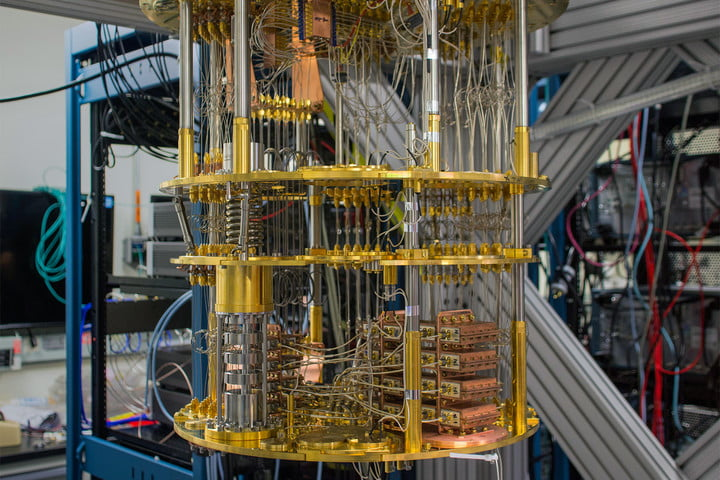
\includegraphics[width=0.8\linewidth]{ibm.jpg}
\captionof{figure}{Ein Quantencomputer von IBM\cite{IBM}}
\end{center}\vspace{1cm}

\subsection*{Paper-Prototyping}
Beim Paper-Prototyping wird ein Prototyp aus einfachsten Mittel hergestellt um eine Software oder eine Hardware zu simulieren. Dazu können verschiedene Komponenten aus Papier hergestellt und auf eine Fläche gelegt werden. Eine Testperson kann sich anschließen durch diesen Prototypen arbeiten in dem ein wissenschaftlicher Mitarbeiter die Logik des Programms imitiert und Komponenten je nach Reaktion der Testperson hinzugefügt, entfernt oder ändert.
\begin{center}\vspace{1cm}
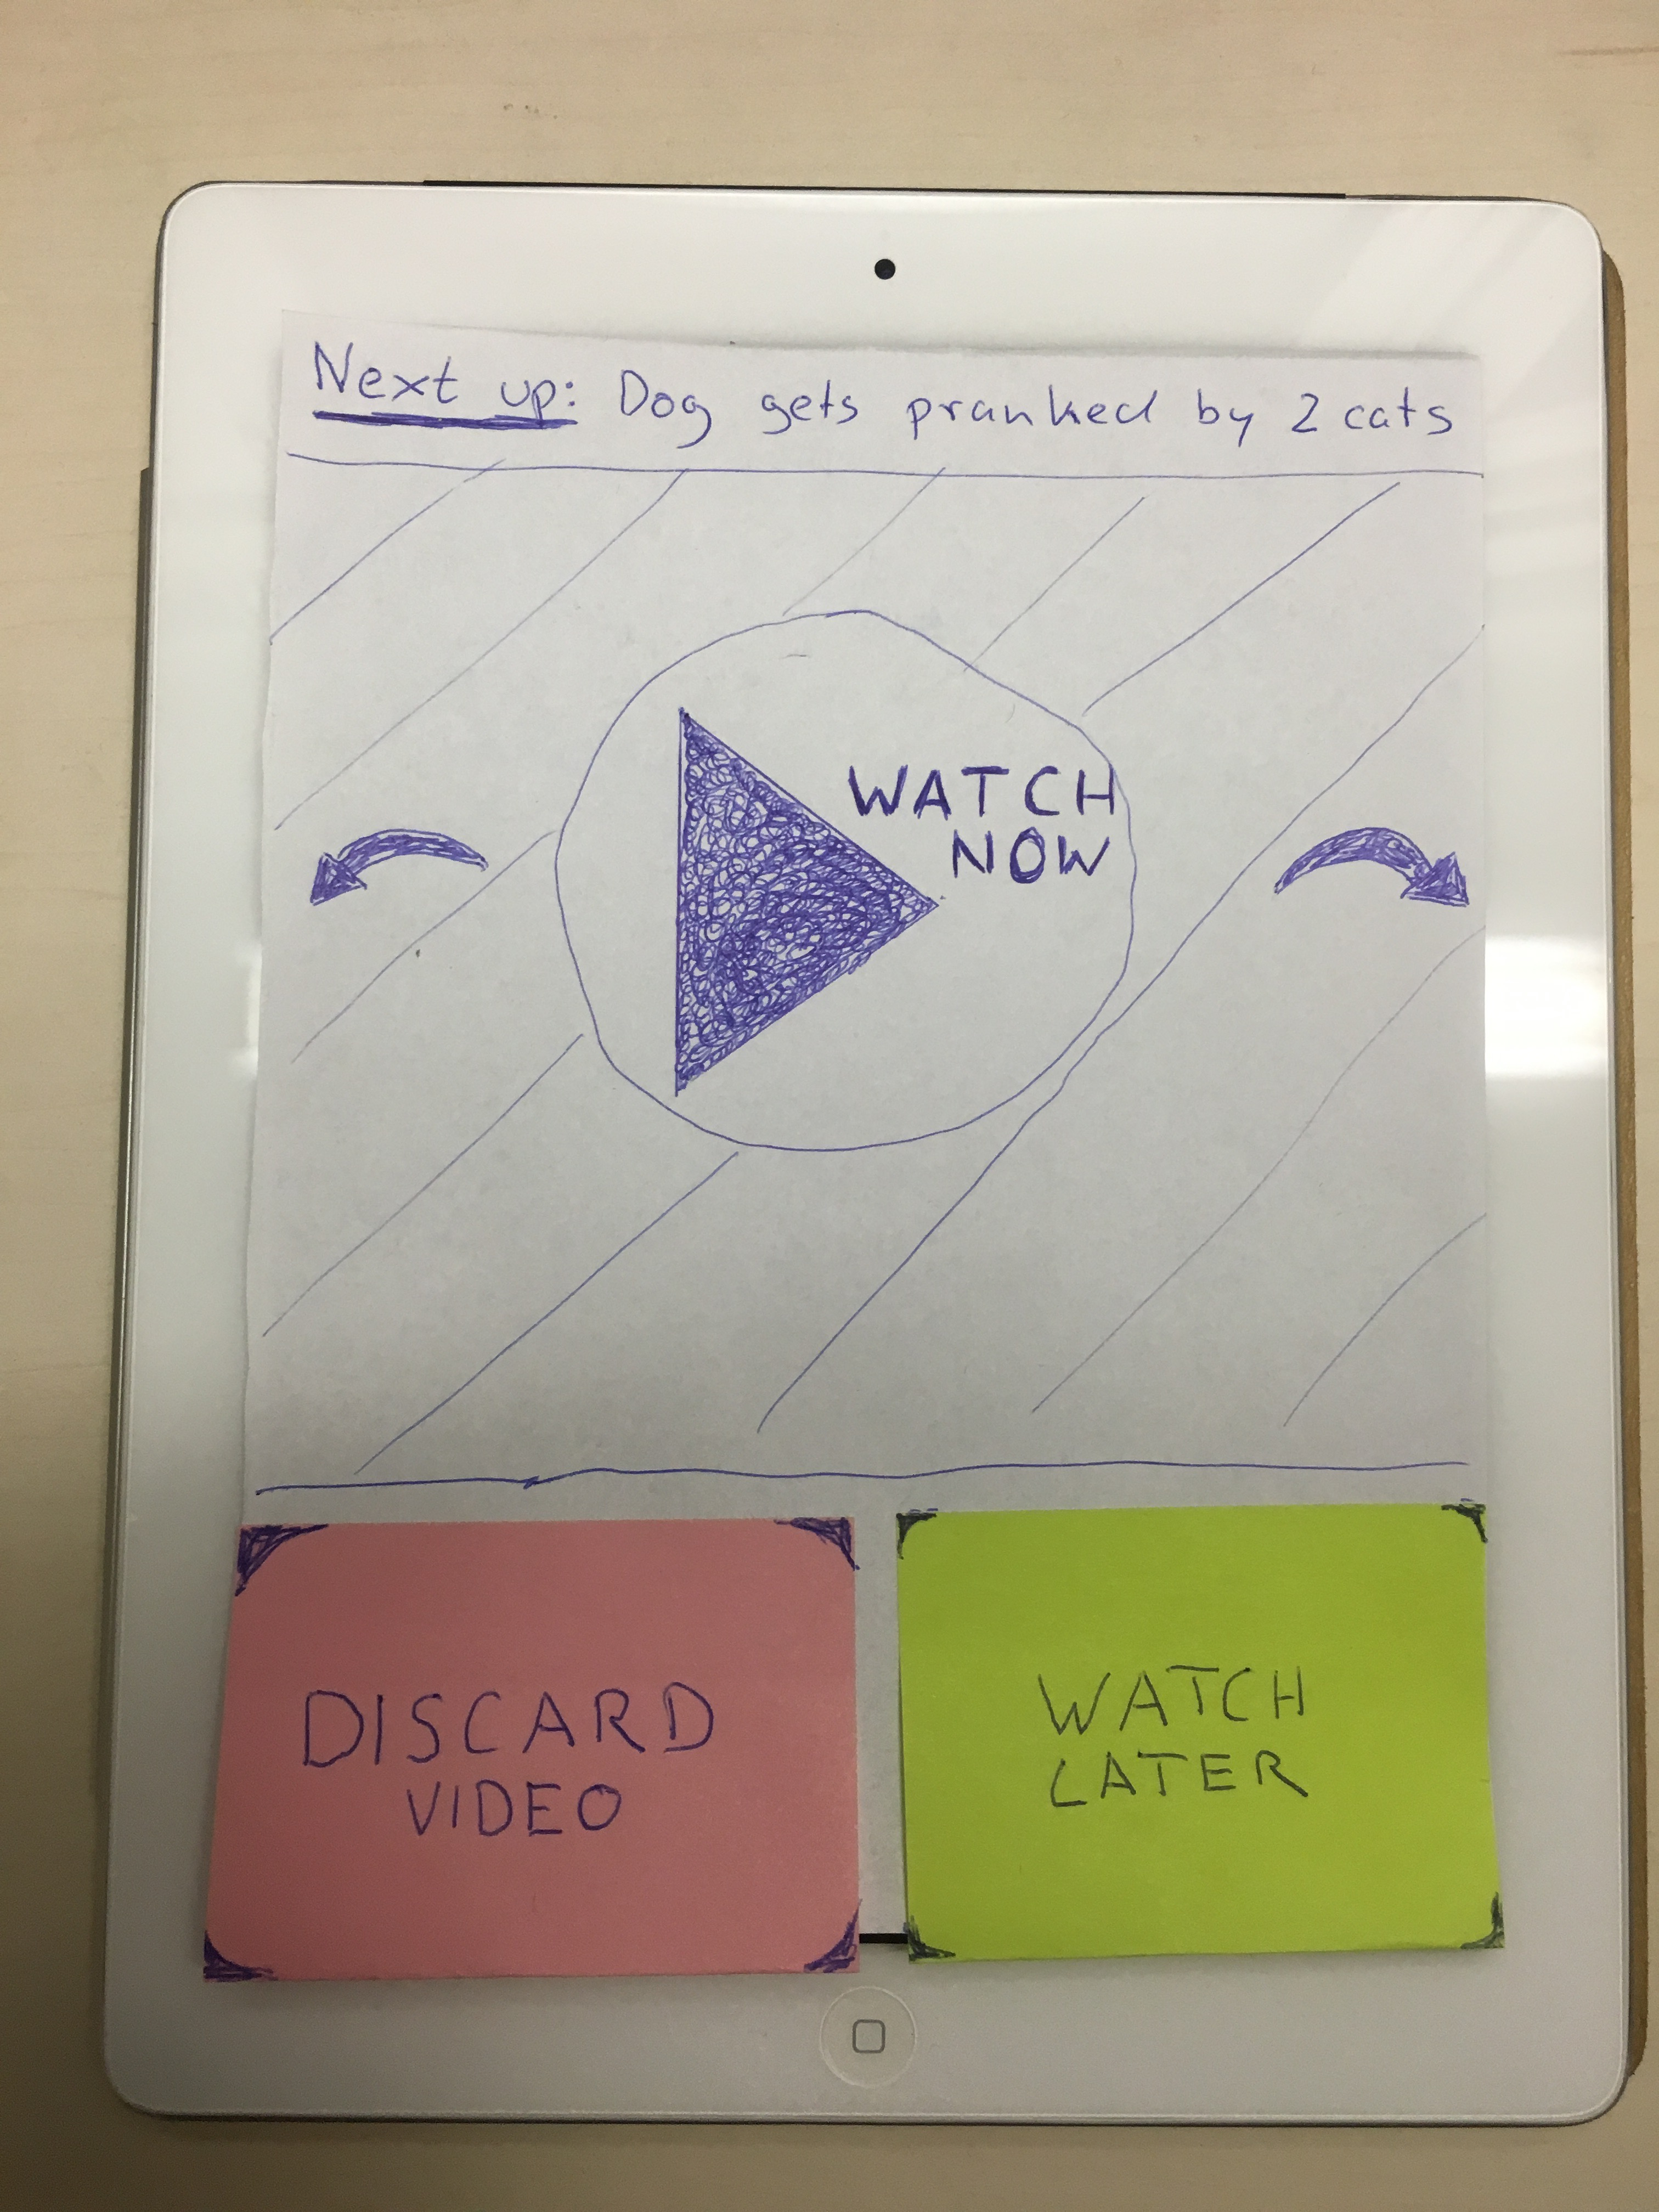
\includegraphics[width=0.8\linewidth]{paper-prototype.jpg}
\captionof{figure}{Ein Beispiel für einen Papier-Prototypen\cite{PAPER}}
\end{center}\vspace{1cm}

\nocite{*} % Print all references regardless of whether they were cited in the poster or not
\printbibliography{}
\end{multicols}
\end{document}
